\documentclass[10pt]{article}
\usepackage[margin=0.8in]{geometry}
\usepackage{amsmath,amssymb,graphicx,longtable,booktabs}
\usepackage[T1]{fontenc}
\usepackage{lmodern}
\usepackage{microtype}
\setlength{\parindent}{0pt}
\setlength{\parskip}{5pt}
\setlength{\emergencystretch}{3em}
\title{Matrix-free factor-TDVP\\Force acceleration and remaining accuracy limits}
\author{Canonical purification dynamics research}
\date{November 14, 2026}
\begin{document}
\maketitle

Reproduction commands · Continuation handoff

The original density-residual factor force can be accelerated without building
its exponentially tall Jacobian. The implementation here uses compact real
one-site tangent coordinates and MPO-output LSQR. On the correlated mixed-chain
D force benchmark, measured speedups over the explicit solver are 3.59, 5.36,
and 27.12 at three, four, and six spins, respectively. Relative factor-velocity
differences are below 4e-9 in these controls. This does \textbf{not} establish a
competitive end-to-end alternative to root TDVP or positive-witness correction.
The interacting-loss case exposes a serious small-population accuracy limit.

All results here are newly executed, finite measurements. The benchmark branch
at \texttt{facc0b7} was cloned, and the existing accelerated branch at the same commit
was continued. Earlier source and numerical tables are preserved. The only
changes to the original factor driver are optional solver injection points;
its default remains the explicit solver.

\section*{Real-linear differential and adjoint}

Let $X=HH^\dagger$, $D_H(K)=KH^\dagger+HK^\dagger$, and
$G=\mathcal L(X^2)$. The original objective is

\[
\min_{K\in T_H\mathcal M_\chi}\|\mathcal J_H(K)-G\|_F^2,
\qquad \mathcal J_H(K)=XD_H(K)+D_H(K)X.
\]

Use the real inner product $\langle A,B\rangle_{\mathbb R}=\mathrm{Re}\,\mathrm{Tr}(A^\dagger B)$.
The image of the Jacobian is Hermitian. For arbitrary complex residual $R$,
only $R_h=(R+R^\dagger)/2$ contributes. Self-adjointness of the Sylvester map
and a cyclic trace give

\[
\begin{aligned}
\langle R,\mathcal J_H(K)\rangle_{\mathbb R}
&=\langle XR_h+R_hX,KH^\dagger+HK^\dagger\rangle_{\mathbb R}\\
&=\langle 2(XR_h+R_hX)H,K\rangle_{\mathbb R}.
\end{aligned}
\]

Thus

\[
\boxed{\mathcal J_H^*(R)=2(XR_h+R_hX)H.}
\]

For Hermitian residuals this is the requested adjoint. Tests use complex,
non-Hermitian factors, velocities and residuals; treating this map as
complex-linear would fail those tests.

\section*{Compact tangent coordinates and MPO-output LSQR}

Canonicalize the factor once per force evaluation. At each nonfinal site take
the orthogonal complement of the left-isometric tensor, coupled to a
right-isometric suffix. The final site is unrestricted. These give the same
orthonormal tangent basis as the explicit solver, but no individual full-chain
basis MPO is stored. Real and imaginary local coordinates are interleaved.

Encoding a residual contracts two environments and the local complement.
Decoding all coordinates uses a block-triangular MPO of bond at most twice the
factor bond. Independent tests compare encoding/decoding with the original
explicit basis and existing tangent projector, including restricted bonds.
Canonical frames are reused throughout each solve; environments involving a
new residual are recomputed. They are not incorrectly reused across changed
residuals or time steps.

Golub-Kahan LSQR acts on this real coordinate space and an MPO codomain. It
uses Jacobian/adjoint applications, MPO sums, norms and compression, with no
physical output arrays of length $4^N$ and no assembled normal matrix. Optional
damping uses an augmented coordinate block rather than explicitly forming
normal equations. The implementation recomputes the stationarity residual at
predicted convergence, periodically, and on exit. Its criterion is

\[
\frac{\|B^*\mathcal J_H^*(\mathcal J_H(Bc)-G)+\lambda^2c\|_2}
{\|B^*\mathcal J_H^*G\|_2}\leq\varepsilon.
\]

Here $B$ is the tangent isometry and $\lambda=0$ by default. Zero-force cases
are handled separately. The default tolerance is 1e-8; this is \textbf{not equivalent}
to the original SVD cutoff \texttt{rcond=1e-11}. The returned diagnostics distinguish
normal residual, physical force residual, iterations, work bonds, products,
local discards and normalization correction. The LSQR condition estimate is a
bidiagonal estimate, not the full Jacobian condition number.

\subsection*{Truncation and failure semantics}

MPO rounding is nonlinear. LSQR's exact-arithmetic guarantees therefore apply
only when these operations accurately represent the fixed linear map. Strict
mode rejects excessive relative discard in any operation and nonconvergence;
near-cancellation sums use an operand scale to avoid treating floating-point
cancellation as a material bond loss. These local checks are useful guards,
not a propagated global error certificate or a proof of adjointness after
arbitrary truncation. The stationarity check uses the same rounded arithmetic;
small dense independent velocity checks are essential evidence in the present
study. \texttt{strict=False} exists for diagnosis and is not used to silently accept
unsafe trajectories. General compressed-Krylov convergence remains open.

A matrix-free force does not make the entire driver matrix-free. The inherited
support audits, generic finite-channel bridge and small-chain scoring remain
dense. No generic large-chain rank-changing trajectory is claimed.

\section*{Gauge, conditioning, and controlled changes of objective}

Right-unitary variations $K=H\Omega$, with $\Omega^\dagger=-\Omega$, are null.
Zero-start, unscaled LSQR selects the minimum-norm tangent solution in exact
arithmetic. This removes only null directions present inside the restricted
tangent. The unrestricted horizontal condition
$H^\dagger K=K^\dagger H$ need not be attainable without changing that tangent.

For a positive diagonal factor, the nonzero singular values are
$\sqrt{2}(h_a^2+h_b^2)^{3/2}$, including $4h_a^3$ on diagonal modes. Hence

\[
\kappa(\mathcal J_H|_{\mathrm{horizontal}})
=\left(\frac{p_{\max}}{p_{\min}}\right)^{3/4}.
\]

The root Sylvester equation has extremal condition
$(p_{\max}/p_{\min})^{1/2}$. Thus explicit column construction is avoidable,
but the factor map has a genuine additional small-population amplification.
Removing exact gauge zeros cannot remove it. Four dense qubit checks in
ablations.json reproduce conditions from 2.83 to
3343.65. Column scaling cuts three/four iterations to two in these tiny oracles;
constructing that scaling from full columns is not a scalable preconditioner.
The production interface accepts a positive diagonal coordinate preconditioner
but does not claim to construct a generally useful one automatically.

A seeded two-spin, bond-two restricted-tangent ablation gives:

\begingroup\small\setlength{\tabcolsep}{3pt}\begin{longtable}{p{0.21\linewidth}p{0.21\linewidth}p{0.21\linewidth}p{0.21\linewidth}}\toprule
Objective & Density residual & Root-velocity residual & Horizontal defect \\
\midrule\endhead
Original density residual & 0.0900053 & 0.163050 & 0.789578 \\
Add horizontal penalty, weight 1 & 0.187857 & 0.275989 & 0.149643 \\
Add velocity ridge, damping 0.01 & 0.0900058 & 0.163025 & 0.787868 \\
Root-velocity residual & 0.110548 & 0.151467 & 0.743018 \\
\bottomrule\end{longtable}\endgroup

The penalty improves its targeted gauge defect while worsening the physical
fit. The root metric improves its targeted root-velocity fit while worsening
the density residual. These are controlled \textbf{different variational methods},
not faster equivalent versions of the original method. The root force in this
ablation comes from a dense Sylvester oracle; it is not used in production
factor evolution. This single-state experiment does not establish trajectory
superiority for either alternative.

Warm starts are supported as coordinates in the current canonical frame;
previous velocities must be projected into it. Recycling has not been benchmarked
as an acceleration result. Local ALS/DMRG sweeps could solve site-effective real
least-squares problems with cached environments, but local stationarity need not
imply global tangent stationarity. No untested sweep solver or automatic
adaptive two-site/bond-growth controller is presented as implemented.

\section*{Independent profiling and force equivalence}

A separate six-spin explicit D force profile took 18.10 seconds: 17.37 seconds
in Jacobian application, approximately 96\%; cumulative compression took 15.09
seconds and the final \texttt{lstsq} only 0.086 seconds. The 416 real columns reproduce
the architectural bottleneck independently. Cumulative profiler categories
overlap and must not be added.

The final paired force measurements, with profiling enabled for both methods,
are in forces\_corrected\_timing.

\begingroup\small\setlength{\tabcolsep}{3pt}\begin{longtable}{p{0.16299999999999998\linewidth}p{0.16299999999999998\linewidth}p{0.16299999999999998\linewidth}p{0.16299999999999998\linewidth}p{0.16299999999999998\linewidth}}\toprule
Spins & Explicit force (s) & MPO-LSQR force (s) & Speedup & Relative velocity difference \\
\midrule\endhead
3 & 0.2473 & 0.0690 & 3.59 & 1.94e-14 \\
4 & 0.8386 & 0.1564 & 5.36 & 2.02e-9 \\
6 & 14.827 & 0.5467 & 27.12 & 3.83e-9 \\
\bottomrule\end{longtable}\endgroup

Use \texttt{force\_total\_seconds}, which includes setup inside the solver, for this
comparison. \texttt{solve\_seconds} excludes that setup. Timing runs request one BLAS
thread and use isolated worker processes; host load, profiling and hardware
still affect observations. They are not repeated-sample confidence intervals.
Preliminary runs are retained and identified, not mixed into the final frontier.

\section*{Scaling scope and bond costs}

A separate analytic product-path test constructs factors, generators and an
exact product-rule factor derivative entirely as MPOs. Force checks complete
at N=3,4,6,8,12,16,32,64 with global relative Frobenius velocity error below
5e-14 in the initial recorded sweep. This establishes the absence of mandatory
exponential output vectors on that structured family. It is a \textbf{force-only}
test with no correlations, integration, rank events or endpoint certification.
The final sweep and its source hash are kept in \texttt{results/product\_scaling\_final}.

At bounded bonds, tangent coordinates occupy order $N\chi_H^2$ numbers, while
Krylov MPOs occupy order $Nw^2$ numbers for work bond $w$. The frames and local
complements have polynomial bond storage. Products have multiplicative raw
bonds before QR/SVD compression, so there is no small universal exponent in a
single declared bond. In particular root and density bonds can grow as
$\chi_H^2$ and $\chi_H^4$. Runtime depends on iteration count, truncation,
physical conditioning and intermediate bonds, not N alone.

Each fixed-bond contraction sweep is linear in N, but this implementation
applies N individual local jumps using separate chain sweeps; generator setup
can therefore be quadratic in N. The product-path timing should not be fitted
to a linear generic trajectory claim. Summed local superoperator MPOs and
zip-up products are concrete next optimizations, subject to residual checks.

\section*{Positivity, rank opening and certification}

Factor retraction continues to normalize $\mathrm{Tr}[(HH^\dagger)^2]=1$,
not the Frobenius norm of H. Positivity survives any factor truncation, but
physical support and accuracy need not. Both force stages and the endpoint
retain the original audits. Tests cover first-order, repeated and delayed
opening, positive finite-channel bridges, unresolved tiny sectors, and guarded
failure after truncation loses support. Fixed-grid evolution has no general
adaptive stability guarantee.

For a valid independent reference $\rho>0$, $S=\sqrt\rho$,
$E=X^2-\rho$ and $M\succeq\rho^{-1}$,

\[
\|X-S\|_F\leq\sqrt{\mathrm{Tr}(E^\dagger EM)},\qquad X=HH^\dagger.
\]

Indeed, for $D=X-S$, $XD+DS=E$. In the left-X/right-S eigenbases every
entry is divided by $x_i+s_j\geq s_j$, proving the inverse-weighted bound.
Unlike a separate stored root, factor X has exactly zero witness defect, so
there is no $2\eta$ term or witness fitting for this purpose. Independent
physical-density and inverse-metric information is still needed.

If an approximate density has trace-norm error at most delta and M bounds the
inverse of the \textbf{true} density, the extra allowance is at most
$\delta\sqrt{\|M\|_{\mathrm{op}}}$. An inverse of an approximate reference is
not automatically a valid bound. If a Hermitian approximate metric differs
from a valid metric by operator norm epsilon, adding epsilon I restores an
upper allowance; its squared weighted-error contribution is at most
$\epsilon\|E\|_F^2$. Without such hypotheses these are diagnostics, not certified
bounds. Ordinary floating-point evaluation here has no rigorous roundoff enclosure.

The dense certificate ablation confirms the inequality for three perturbation
scales and separates inverse-reference, weighted-contraction and redundant
witness-check costs. It excludes witness fitting and cannot establish a total
certification advantage. Native witness timings separately expose reference,
prediction, correction and endpoint audit calls; overlapping nested categories
must not be summed. Native end-to-end time remains authoritative.

\section*{Trajectory comparisons and scientific conclusions}

The final trajectory, matched-grid and stress tables and figures below are
produced from saved worker outputs. They compare the raw global canonical-root
Frobenius error, not local marginal agreement. Conventional root evolution,
positive-witness evolution and predictor-free endpoint correction are distinct
methods. The latter two have independent physical reference information and
may correct errors; direct factor evolution has no such endpoint correction.

For D3, positive-witness controls use the same uniform 5/10/20-step endpoint
grids as the factor/root controls, at requested certificate tolerances
1e-3, 1e-5 and 1e-7. Native historical-grid witness results are retained separately.
A cost frontier selects only actually completed runs at the same family, size
and final time. Different step counts may win at different accuracy targets;
these are minimum \textbf{observed} costs, not exhaustive optimized complexities.

\subsection*{Measured global trajectories and costs}

\begingroup\small\setlength{\tabcolsep}{3pt}\begin{longtable}{p{0.13166666666666665\linewidth}p{0.13166666666666665\linewidth}p{0.13166666666666665\linewidth}p{0.13166666666666665\linewidth}p{0.13166666666666665\linewidth}p{0.13166666666666665\linewidth}}\toprule
Family & N & Steps & Method & Global CP error & Total seconds \\
\midrule\endhead
A & 3 & 10 & matrix\_free & 0.000701494 & 1.479 \\
A & 3 & 10 & root & 0.000968621 & 0.3484 \\
B & 3 & 10 & matrix\_free & 0.000701494 & 1.457 \\
B & 3 & 10 & root & 0.000968621 & 0.1001 \\
C & 3 & 10 & matrix\_free & 8.61868e-06 & 0.397 \\
C & 3 & 10 & root & 1.53041e-05 & 0.09574 \\
E & 3 & 10 & matrix\_free & 0.000231632 & 0.4476 \\
E & 3 & 10 & root & 0.000196362 & 0.1008 \\
F\_loss & 3 & 10 & matrix\_free & 0.00427466 & 1.766 \\
F\_loss & 3 & 10 & root & 1.33834e-05 & 0.1165 \\
F\_delayed & 1 & 10 & matrix\_free & 0.000218469 & 0.07123 \\
F\_delayed & 1 & 10 & root & 6.36213e-06 & 0.07959 \\
D & 3 & 20 & matrix\_free & 5.69795e-08 & 2.092 \\
D & 3 & 20 & root & 5.66922e-08 & 0.1309 \\
D & 4 & 20 & matrix\_free & 6.95208e-08 & 7.086 \\
D & 4 & 20 & root & 6.91869e-08 & 0.1745 \\
\bottomrule\end{longtable}\endgroup

At D3 target global CP error 1e-7, the minimum observed end-to-end costs are:

\begingroup\small\setlength{\tabcolsep}{3pt}\begin{longtable}{p{0.28833333333333333\linewidth}p{0.28833333333333333\linewidth}p{0.28833333333333333\linewidth}}\toprule
Method & Global CP error & Total seconds \\
\midrule\endhead
Conventional root TDVP & 5.66922e-8 & 0.130875 \\
Accelerated direct factor TDVP & 5.69795e-8 & 2.09189 \\
Positive-witness root TDVP & 3.08755e-9 & 0.096866 \\
Positive-factor correction without predictor & 2.06052e-9 & 0.046660 \\
\bottomrule\end{longtable}\endgroup

These are minimum costs over the executed uniform-grid settings, not the same
winning number of steps for every method. All methods had the same available
5/10/20-step grids. Correction methods additionally use independent density and
inverse-metric information. Worker totals exclude interpreter/import startup;
\texttt{subprocess\_seconds} includes it. Certificate and reference costs are included,
but native checkpoint I/O and internal scoring also contribute to witness totals.
No claim of a predictor speed advantage follows from the correction results.

In the E3 ten-step grid, factor/root errors remain above 1e-5. Supplementary
native-grid E witness runs do meet tighter targets, but are not inserted into
the primary same-grid frontier. Empty E witness entries in that frontier mean
not included in this comparison, not failure to attain an error in all runs.

Tilted C here is a three-spin boundary control. Historical C4/C8 half-Petz and
local-unitary active-window results are retained in the preceding comparison
report; they cannot be substituted as same-size matched-resource measurements
for this C3 trajectory. A/B long-time and generic larger correlated trajectory
claims are not established by this limited finite-grid experiment.

\subsection*{Interacting-loss negative result}

Identical F\_loss3 settings (ten intervals to 0.03, factor/work caps four) give:

\begingroup\small\setlength{\tabcolsep}{3pt}\begin{longtable}{p{0.28833333333333333\linewidth}p{0.28833333333333333\linewidth}p{0.28833333333333333\linewidth}}\toprule
Solver & Global CP error & Total seconds \\
\midrule\endhead
Explicit SVD & 5.94226e-5 & 2.9624 \\
MPO-LSQR, tolerance 1e-8 & 4.27466e-3 & 1.7469 \\
MPO-LSQR, tolerance 1e-10 & 1.58697e-4 & 5.0571 \\
MPO-LSQR, tolerance 1e-12 & 1.58153e-4 & 8.2971 \\
\bottomrule\end{longtable}\endgroup

The explicit Jacobian condition reaches approximately 1.09e8. At tolerance
1e-12 the density error (5.76872e-5) nearly matches the explicit density error
(5.76873e-5), but the canonical-root errors differ substantially. Small
populations amplify discrepancies at the root scale. LSQR has no full
reorthogonalization or rank-revealing cutoff equivalent to SVD, and small normal
residual is not a small velocity error guarantee. Tightening stationarity alone
is therefore insufficient. This is a preserved unsuccessful accuracy experiment,
not evidence that the methods are equivalent near a singular boundary.

Intermediate Krylov residuals are excluded from accepted-force maximum fields;
postprocessing notes document that correction to diagnostic aggregation. This
did not change numerical trajectories or measured timings.

\begin{center}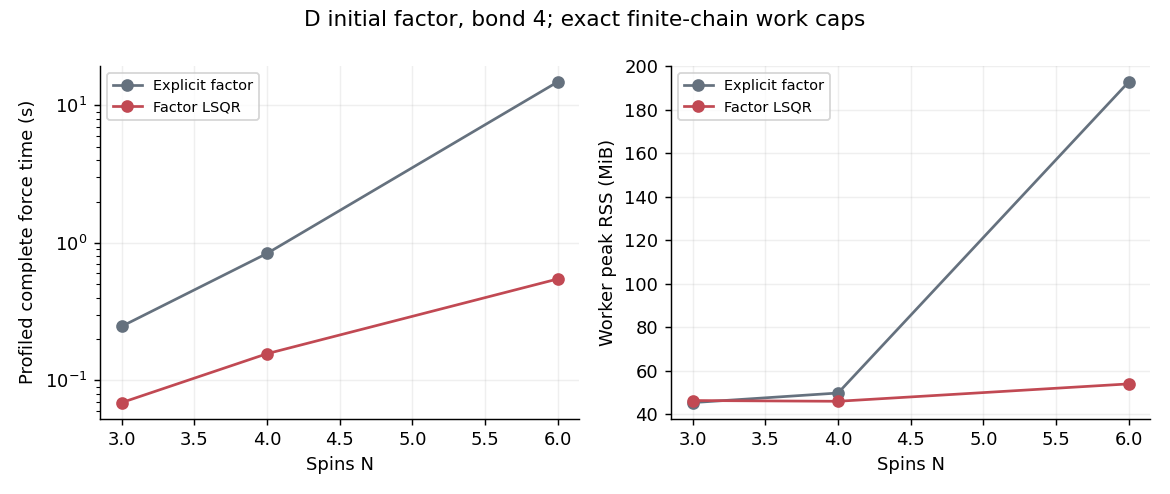
\includegraphics[width=\linewidth,height=.52\textheight,keepaspectratio]{figures/force_scaling.png}\end{center}
\begin{center}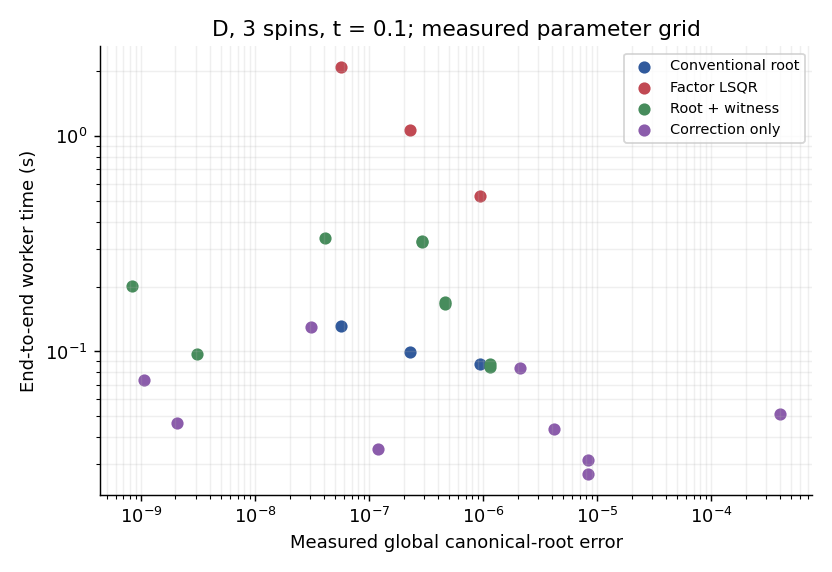
\includegraphics[width=\linewidth,height=.52\textheight,keepaspectratio]{figures/accuracy_runtime.png}\end{center}
\begin{center}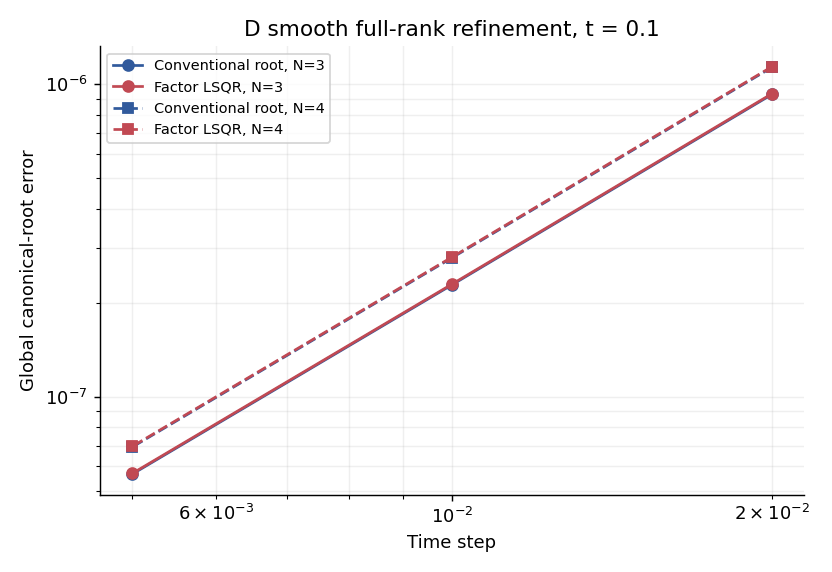
\includegraphics[width=\linewidth,height=.52\textheight,keepaspectratio]{figures/step_convergence.png}\end{center}
\begin{center}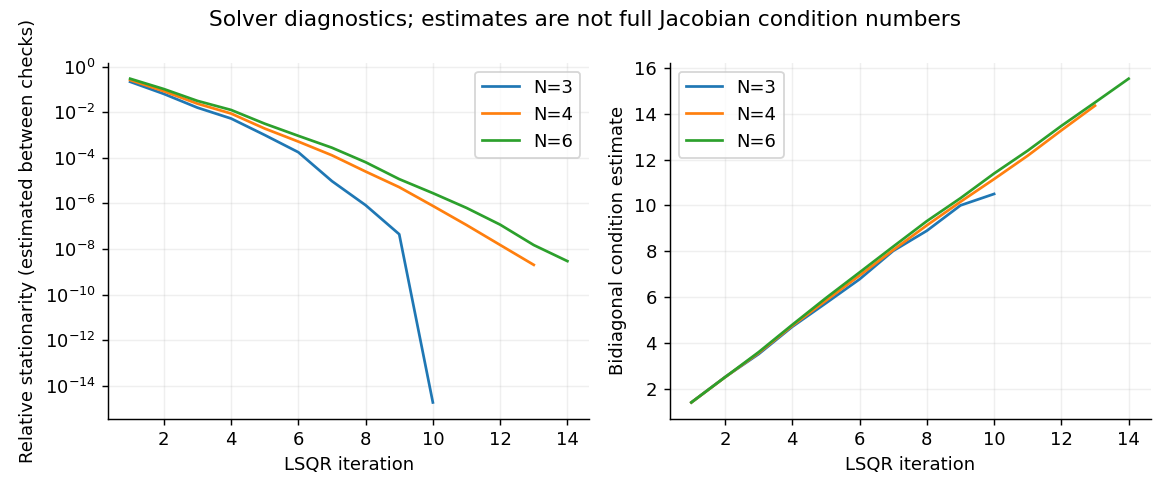
\includegraphics[width=\linewidth,height=.52\textheight,keepaspectratio]{figures/conditioning.png}\end{center}

\clearpage
\subsection*{Answers to the ten research questions}

\par\noindent 1. \textbf{Implementation artifact?} Explicit column construction is a major avoidable
   cost: the six-spin force is about 27 times faster here. Remaining dynamics,
   conditioning and representation costs prevent attributing the whole slowdown
   to that artifact.
\par\noindent 2. \textbf{Remove exponential Jacobian output?} Yes in the production force. The
   no-dense regression and MPO-only product tests verify it. Dense rank handling
   still limits generic end-to-end evolution.
\par\noindent 3. \textbf{Observed complexity?} The tables show measured sizes, bonds, iterations,
   memory and timings. Fixed-bond contractions are polynomial, and separate local
   jump sweeps add quadratic setup work. No generic size/condition power law is
   inferred from three correlated force sizes and one product family.
\par\noindent 4. \textbf{Intrinsically harder than root Sylvester?} In full-space spectral scaling,
   the factor Jacobian amplifies population ratios to power 3/4 rather than 1/2.
   Restricted tangents, null spaces and bond growth can further change difficulty.
\par\noindent 5. \textbf{Gauge/preconditioning stability?} Zero-start LSQR handles represented null
   modes. The restricted-tangent penalty ablation demonstrates a tradeoff, not a
   universal cure. No scalable automatic preconditioner or generic stable
   restricted-bond evolution has been established.
\par\noindent 6. \textbf{Cheaper certificate?} Zero witness defect removes fitting/checking that
   defect, but not independent reference or metric propagation. A net total-cost
   advantage is not demonstrated.
\par\noindent 7. \textbf{Competitive at matched CP error?} The measured force speedup does not
   establish an end-to-end win against root evolution or witness correction.
   See the observed-cost frontier and retained failures; correction resources
   remain unequal even on matched grids.
\par\noindent 8. \textbf{Preferable regimes?} The most promising tested setting is a smooth,
   well-conditioned full-rank path with economical factor bonds when positivity
   is needed directly. That is a research direction, not evidence of a winning
   algorithm over the measured baselines.
\par\noindent 9. \textbf{Dominant obstruction?} After removing columns, iteration/compression and
   small-population accuracy remain; generic rank handling and affordable global
   reference/certification are unresolved scalability barriers.
\par\noindent 10. \textbf{Next concrete development?} Build a contraction-based restricted-tangent
    preconditioner with physical-error-aware stopping and adaptive stepping,
    then combine controlled bond growth and scalable support handling. Validate
    against matched global CP error before claiming further speedups.

\section*{Validation and remaining deliverables}

The combined new and predecessor regression run passes \textbf{48 tests} in
tests\_full.log, including 17 new accelerated checks.
The no-dense test patches dense export and explicit basis construction to fail
inside the production solve. Rank-opening checks remain finite-size tests.
See the benchmark manifest for authoritative
versus preliminary datasets, timing interpretation and source provenance.
General local-sweep optimization, adaptive rank/bond/step control, scalable
rank-changing trajectories and a universal certification advantage remain open.
\end{document}
